\section{ Model comparisons}\label{model_comparisons}

As mentioned in section \ref{cnn_ref} we used Keras Tuner model to find hyperparameters that would yield the highest accuracy.
Instead of hard-coding hyperparameters when building a model with Keras API, we defined a search space of possible values with \verb|HyperParameter| class and used that as a hyperparameter.

We then passed the created model to a \verb|RandomSearch| class, with few other parameters such as batch size, number of epochs and maximum number of trials.
We then started hyperparameter search, which means that Keras Tuner was randomly picking a set of hyperparameters and training a model with them. 
This process was repeated for a trial number of times.
Accuracy and hyperparameters that were used while training every module were saved to a log file for later analysis.

After training a number of different models we handpicked a few of them and compared them.
Comparison of equivalent model trained in Edge Impulse studio was also done.


\subsection{ Hyperparameter search space and results analysis}

General structure of CNN model was already described in section \ref{cnn_ref} and in Figure \ref{model_code}.
We decided to search for following hyperparameters: number of filters in all three convolutional layers (can be different for each layer), filter size in all three convolutional layers (same for all layers), size of dense layer, dropout rate and learning rate.
Possible values of hyperparameters (also known as hyperparameter search space) are specified in table \ref{hyper_table1}.

\begin{table}
    \centering
    \caption{ First hyperparameter search space}
    \rowcolors{2}{white}{gray!25}
    \begin{tabular}{@{} *5l @{}}    \toprule
        \textbf{Hyperparameter} & \textbf{Set of values}\\\midrule
        \verb|FilterNum1|       & From 16 to 80, with a step of 8\\ 
        \verb|FilterNum2|       & From 16 to 80, with a step of 8\\ 
        \verb|FilterNum3|       & From 16 to 80, with a step of 8\\
        \verb|FilterSize|       & 3 x 3 or 3 x 4\\
        \verb|DenseSize|        & From 16 to 96, with a step of 8\\
        \verb|DropoutRate|      & From 0.2 to 0.5, with a step of 0.05\\
        \verb|LearningRate|     & 0.0001 or 0.0003\\\toprule
        \textbf{Random search}  & \textbf{value}\\
        \textbf{variable}       & \\\midrule
        \verb|EPOCHS|           & 25\\
        \verb|BATCH_SIZE|       & 100\\
        \verb|MAX_TRIALS|       & 300\\\bottomrule
    \end{tabular}
    \label{hyper_table1}
\end{table}

Search space of \verb|filter_numX|, \verb|dense_size| and \verb|dropout_rate| hyperparameters was chosen based on initial training tests and various models that were trained on similar data.
Value of \verb|filter_size| is usually 3 x 3, however all example ML projects were training on image date of same dimensions.
We wanted to test how would a filter with same ratio of dimensions as image data (3 x 4 and 60 x 80 respectively) perform.
Hyperparameter \verb|learning_rate| was chosen heuristically, we saw that higher values, such as 0.001 or 0.003, would leave model's accuracy stuck at suboptimal optima, from where it could not be improve anymore.

We also had to set 3 variables that directly affected how long will random search last.
From initial tests we saw that models usually reached maximum possible accuracy around \nth{20} epoch, to give some headroom we set the number of epochs to 25.
We kept batch size relatively small, at 100, which meant that weights would get updated regularly.
Hyperparameter \verb|MAX_TRIALS| had the biggest impact on the training time, we set it to 300.

Training lasted for about 12 hours. 
After it was done we compiled a list of all 300 trained models and their different hyperparameter values, number of parameters and accuracies, part of it can be seen in Table \ref{hyper_results1}.

\begin{table}
    \centering
    \caption{ Partial results of first random search of hyperparameters}
    \rowcolors{2}{gray!25}{white}
    \begin{tabular}{llllllllrl}
        \textbf{Hyperparameter} & \rot{FilterNum1} & \rot{FilterNum2} & \rot{FilterNum3} & \rot{DenseSize} & \rot{DropoutRate}  &\rot{FilterSize} & \rot{LearningRate} & \rot{Number of parameters} & \rot{Accuracy[\%]}  \\\toprule
        \textbf{Model ID} &&&&&&&&\\\toprule
        0a & 72 & 80 & 64 & 72 & 0.4  & 3x4 & 0.0003 & 1.514,400 & 98.35\\
        1a & 32 & 40 & 72 & 56 & 0.35 & 3x4 & 0.0001 & 1.260,332 & 98.31\\
        2a & 40 & 48 & 32 & 64 & 0.35 & 3x4 & 0.0001 &   656,797 & 98.31\\
        3a & 56 & 16 & 48 & 72 & 0.4  & 3x4 & 0.0001 & 1,057,924 & 98.28\\
        4a & 80 & 64 & 40 & 96 & 0.45 & 3x4 & 0.0003 & 1,245,788 & 98.28\\
        5a & 64 & 24 & 72 & 88 & 0.45 & 3x3 & 0.0001 & 1,931,356 & 98.28\\
        6a & 64 & 56 & 40 & 80 & 0.35 & 3x3 & 0.0001 & 1,013,556 & 98.24\\
        7a & 16 & 40 & 64 & 88 & 0.35 & 3x3 & 0.0003 & 1,719,108 & 98.24\\
        8a & 48 & 64 & 32 & 64 & 0.35 & 3x4 & 0.0003 &   676,884 & 98.24\\
        9a & 72 & 48 & 56 & 80 & 0.3  & 3x4 & 0.0001 & 1,419,172 & 98.24\\\midrule
       91a & 72 & 48 & 56 & 40 & 0.35 & 3x3 & 0.0003 &   728,324 & 98.00\\
       92a & 48 & 24 & 64 & 64 & 0.35 & 3x4 & 0.0001 & 1,262,092 & 98.00\\
       93a & 24 & 48 & 32 & 72 & 0.4  & 3x3 & 0.0001 &   716,076 & 98.00\\
       94a & 32 & 48 & 72 & 32 & 0.25 & 3x3 & 0.0001 &   736,732 & 98.00\\
       95a & 64 & 24 & 64 & 48 & 0.3  & 3x4 & 0.0001 &   959,628 & 98.00\\
       96a & 16 & 32 & 72 & 80 & 0.25 & 3x4 & 0.0001 & 1,762,508 & 98.00\\
       97a & 72 & 56 & 40 & 56 & 0.45 & 3x4 & 0.0003 &   748,580 & 98.00\\
       98a & 32 & 24 & 24 & 48 & 0.35 & 3x3 & 0.0001 &   358,308 & 98.00\\
       99a & 48 & 16 & 40 & 40 & 0.45 & 3x3 & 0.0003 &   493,412 & 98.00\\
      100a & 24 & 72 & 64 & 40 & 0.45 & 3x3 & 0.0003 &   844,684 & 98.00\\\midrule
      191a & 64 & 56 & 16 & 52 & 0.4  & 3x3 & 0.0001 &   386,996 & 97.76\\
      192a & 48 & 40 & 24 & 24 & 0.4  & 3x4 & 0.0001 &   208,172 & 97.73\\
      193a & 56 & 64 & 72 & 24 & 0.25 & 3x4 & 0.0003 &   617,692 & 97.73\\
      194a & 48 & 72 & 48 & 32 & 0.25 & 3x4 & 0.0003 &   544,652 & 97.73\\
      195a & 72 & 56 & 24 & 56 & 0.25 & 3x4 & 0.0003 &   469,012 & 97.73\\
      196a & 72 & 48 & 72 & 40 & 0.3  & 3x3 & 0.0003 &   927,252 & 97.73\\
      197a & 80 & 16 & 32 & 80 & 0.25 & 3x3 & 0.0001 &   785,380 & 97.73\\
      198a & 56 & 24 & 16 & 88 & 0.25 & 3x3 & 0.0001 &   438,996 & 97.73\\
      199a & 56 & 24 & 16 & 88 & 0.25 & 3x3 & 0.0001 &   438,996 & 97.73\\\midrule
      295a & 48 & 32 & 64 & 16 & 0.5  & 3x4 & 0.0001 &   351,012 & 95.87\\
      296a & 40 & 24 & 56 & 24 & 0.5  & 3x4 & 0.0001 &   431,572 & 95.77\\
      297a & 56 & 16 & 80 & 16 & 0.2  & 3x4 & 0.0001 &   411,020 & 95.63\\
      298a & 24 & 16 & 48 & 24 & 0.5  & 3x4 & 0.0001 &   359,924 & 94.46\\
      299a & 40 & 48 & 56 & 16 & 0.35 & 3x3 & 0.0003 &   310,860 & 82.86\\\bottomrule
    \end{tabular}
    \label{hyper_results1}
\end{table}

It is important to keep in mind that we are dealing with imbalanced dataset, where 82.86 \% of our validation data are elephant images.
Simply classifying all images as elephant class would yield 82.86 \% accuracy, which sounds high, although it is actually not helpful.

After analyzing results we came to several conclusions:

\begin{enumerate}
    \item We saw that almost all trained models, except of the last one, achieved accuracy above 90 \%. This proved that the general architecture of the model was appropriate for the problem.
    \item We could not see any visible correlation between a specific choice of a certain hyperparameter and accuracy. This shows that selection of hyperparameters is really a non-heuristic task.
    \item Filter of size 3 x 4 did not perform significantly better compared to one with size 3 x 3. 
    \item There is a weak correlation between number of parameters (model's complexity) and accuracy. Although eight of top ten models have more then 1 million parameters, models with IDs 2 and 8 have almost half of the parameters, but still perform well.
    \item First 200 models cover an accuracy range of 0.62 \%. However inside of this range model number of parameters varies hugely, for example, model with ID \textit{192a} has more than 8 times less parameters than model than model with ID \textit{96a}, although the difference in accuracy (0.27 \%) is negligible.
\end{enumerate}

As we realized that we do not need complex models to achieve high accuracy on our training data, we decided to run the random search of hyperparameters again.
We decided to lower the maximum and minimum numbers of filters and size of dense layer.
We also decreased the step from 8 to 2.
We decided to lower the bottom boundary of \verb|DropoutRate| from 0.2 to 0.0, which means that some models will not be using dropout layer at all.
We expected that training without dropout layer would produce suboptimal results, however we wanted to test it.
Redefined search space for second random search can be seen in Table \ref{hyper_table2}
We increased the number of \verb|MAX_TRIALS| from 300 to 500, as we were expecting that more models will end up underfitting and also because there would be more possible options because of smaller step size.

\begin{table}
    \centering
    \caption{ Second hyperparameter search space}
    \rowcolors{2}{white}{gray!25}
    \begin{tabular}{@{} *5l @{}}    \toprule
        \textbf{Hyperparameter} & \textbf{Set of values}\\\midrule
        \verb|FilterNum1|       & From 4 to 48, with a step of 2\\ 
        \verb|FilterNum2|       & From 4 to 48, with a step of 2\\ 
        \verb|FilterNum3|       & From 4 to 48, with a step of 2\\
        \verb|FilterSize|       & 3 x 3 or 3 x 4\\
        \verb|DenseSize|        & From 4 to 48, with a step of 2\\
        \verb|DropoutRate|      & From 0.0 to 0.5, with a step of 0.05\\
        \verb|LearningRate|     & 0.0001 or 0.0003\\\toprule
        \textbf{Random search}  & \textbf{value}\\
        \textbf{variable}       & \\\midrule
        \verb|EPOCHS|           & 25\\
        \verb|BATCH_SIZE|       & 100\\
        \verb|MAX_TRIALS|       & 500\\\bottomrule
    \end{tabular}
    \label{hyper_table2}
\end{table}

Partial table of results of random hyperparameter search can be seen in Table \ref{hyper_results2}.

\begin{table}
    \centering
    \caption{ Partial results of second random search of hyperparameters}
    \rowcolors{2}{gray!25}{white}
    \begin{tabular}{llllllllrl}
        \textbf{Hyperparameter} & \rot{FilterNum1} & \rot{FilterNum2} & \rot{FilterNum3} & \rot{DenseSize} & \rot{DropoutRate}  &\rot{FilterSize} & \rot{LearningRate} & \rot{Number of parameters} & \rot{Accuracy[\%]}  \\\toprule
        \textbf{Model ID} &&&&&&&&\\\toprule
        0b & 40 & 20 & 20 & 48 & 0.25 & 3x4 & 0.0001 & 304,216 & 98.14\\
        1b & 44 & 10 & 28 & 42 & 0.2  & 3x4 & 0.0003 & 362,264 & 98.14\\
        2b & 18 & 38 & 26 & 38 & 0.1  & 3x4 & 0.0003 & 316,956 & 98.11\\
        3b & 46 & 34 & 28 & 40 & 0.35 & 3x4 & 0.0003 & 367,056 & 98.07\\
        4b & 26 & 36 & 36 & 34 & 0.15 & 3x4 & 0.0003 & 394,568 & 98.04\\\midrule
       95b & 20 & 16 & 34 & 40 & 0.3  & 3x3 & 0.0003 & 416,230 & 97.62\\
       96b & 46 & 42 & 28 & 32 & 0.4  & 3x3 & 0.0003 & 297,466 & 97.62\\
       97b & 30 & 26 & 30 & 34 & 0.2  & 3x3 & 0.0001 & 320,570 & 97.59\\
       98b & 20 & 10 & 16 & 46 & 0.45 & 3x3 & 0.0003 & 224,500 & 97.59\\
       99b & 32 & 20 & 32 & 26 & 0.25 & 3x4 & 0.0003 & 265,562 & 97.59\\\midrule
      195b & 28 & 16 & 40 & 24 & 0.1  & 3x3 & 0.0001 & 298,252 & 97.31\\
      196b & 44 & 30 & 32 & 20 & 0.3  & 3x4 & 0.0003 & 220,098 & 97.31\\
      197b & 46 & 40 & 10 & 40 & 0.1  & 3x3 & 0.0001 & 140,874 & 97.31\\
      198b & 12 & 28 & 40 & 32 & 0.4  & 3x4 & 0.0003 & 401,860 & 97.31\\
      199b & 36 & 38 &  6 & 40 & 0.4  & 3x3 & 0.0003 &  86,972 & 97.31\\\midrule
      295b & 20 &  8 & 34 & 26 & 0.3  & 3x3 & 0.0003 & 269,464 & 96.90\\
      296b & 18 & 16 & 10 & 20 & 0.3  & 3x4 & 0.0003 &  65,740 & 96.87\\
      297b &  8 & 22 & 28 & 16 & 0.1  & 3x3 & 0.0001 & 141,742 & 96.87\\
      298b & 18 & 28 & 14 & 32 & 0.25 & 3x4 & 0.0001 & 145,592 & 96.87\\
      299b & 28 & 40 & 20 & 12 & 0.25 & 3x3 & 0.0001 &  89,684 & 96.87\\\midrule
      395b & 10 & 20 & 12 & 30 & 0.0  & 3x3 & 0.0001 & 112,246 & 96.87\\
      396b & 24 & 24 & 46 & 18 & 0.2  & 3x3 & 0.0003 & 263,924 & 96.14\\
      397b &  6 & 18 & 12 & 24 & 0.4  & 3x4 & 0.0001 &  90,520 & 96.11\\
      398b & 44 & 22 &  6 & 32 & 0.45 & 3x4 & 0.0001 &  71,564 & 96.11\\
      399b & 12 & 16 & 10 & 28 & 0.25 & 3x4 & 0.0001 &  88,550 & 96.08\\\midrule
      495b & 32 & 14 & 40 &  8 & 0.5  & 3x4 & 0.0003 & 109,334 & 82.86\\
      496b & 36 & 38 & 22 &  6 & 0.2  & 3x3 & 0.0003 &  59,890 & 82.86\\
      497b & 42 & 30 & 22 &  6 & 0.4  & 3x3 & 0.0003 &  57,386 & 82.86\\
      498b &  4 &  4 & 20 & 12 & 0.4  & 3x3 & 0.0003 &  72,992 & 82.86\\
      499b & 32 & 36 & 36 &  4 & 0.15 & 3x3 & 0.0001 &  65,648 & 82.86\\\bottomrule
    \end{tabular}
    \label{hyper_results2}
\end{table}

Some observations:
\begin{enumerate}
    \item We can see that the accuracy of the best model 0b compared to the best model 0a from previous search is only 0.21 \% lower, although it has about 5 times less parameters.
    \item Although that it might seem that \verb|FilterSize| of 3 x 4 yields best results, we did not saw a strong bias towards on or another option after manually analyzing best 30 models.
    \item We can see that worst five models have the same accuracy of 82.86 \%, same as the worst performing model from first random search. There are 82.86 \% images of elephants in validation class, which means that model probably assigned all validation images to elephant class and was satisfied with achieved accuracy.
    \item We can see that the model with ID \textit{296b} has quite low number of parameters, only 65,740.
\end{enumerate}

After making a skim analysis of results, we decided to go through the whole list of trained results and mark down those with extremely low number of parameters, which can be seen in Table \ref{small_models}.

\begin{table}
    \centering
    \caption{ Partial results of second random search of hyperparameters}
    \rowcolors{2}{gray!25}{white}
    \begin{tabular}{llllllllrl}
        \textbf{Hyperparameter} & \rot{FilterNum1} & \rot{FilterNum2} & \rot{FilterNum3} & \rot{DenseSize} & \rot{DropoutRate}  &\rot{FilterSize} & \rot{LearningRate} & \rot{Number of parameters} & \rot{Accuracy[\%]}  \\\toprule
        \textbf{Model ID} &&&&&&&&\\\toprule
      172b & 42 & 44 &  8 & 14 & 0.1  & 3x4 & 0.0001 &  60,672 & 97.38\\
      230b & 34 &  6 &  4 & 40 & 0.2  & 3x3 & 0.0003 &  50,606 & 97.18\\
      265b &  6 & 46 &  6 & 24 & 0.3  & 3x3 & 0.0003 &  48,404 & 97.01\\
      270b & 36 & 20 & 12 & 10 & 0.15 & 3x3 & 0.0003 &  45,086 & 97.01\\
      304b & 46 &  6 & 10 & 12 & 0.2  & 3x4 & 0.0003 &  40,710 & 96.87\\
      338b &  4 & 18 &  6 & 10 & 0.05 & 3x4 & 0.0003 &  20,290 & 96.63\\
      454b & 10 & 14 &  8 &  6 & 0.05 & 3x4 & 0.0001 &  17,610 & 94.18\\
      460b &  6 & 28 &  4 &  8 & 0.1  & 3x4 & 0.0003 &  13,114 & 93.60\\\bottomrule
    \end{tabular}
    \label{hyper_results2}
\end{table}

\subsection{ Comparison of selected, re-trained models}
    
Two random searches gave us a large amount of different models to choose from.
In every other ML application where the execution time would not be a constraint, we could simply take the best performing model and be done with it.
In our case we need to make a trade off between model's accuracy and execution speed.

For comparison and later on device performance testing we decided to pick and retrain\footnotemark 6 different models: \textit{0a}, \textit{2a}, \textit{0b}, \textit{172b}, \textit{338b} and \textit{460b}.
We chose the models on purpose to vary greatly in number of parameters, as we expected that this will have important effect on the inference time. 

\footnotetext{Retraining was required as Keras Tuner module only saved hyperparameter settings during search and not each trained model.
As the weights are initially randomized accuracy of retrained models is going to be similar but not exact when compared to the accuracy returned by random search.}

As we are dealing with imbalanced dataset, where 82.86 \% of our validation data consists of elephant images, accuracy is not the best metric to use when comparing models.
Precision and recall metrics\footnotemark can give us better idea how well the models are performing, results can bee seen in Table \ref{precision_recall_table}.

\footnotetext{Precision tells us what percentage of data points in a specific predicted class actually fall into that class.
Recall tells us what percentage of data points inside a certain class were actually predicted correctly\cite{geron}.}

\begin{table}
    \centering
    \caption{ Second hyperparameter search space}
    \rowcolors{2}{gray!25}{white}
    \begin{tabular}{ lrrrrrrrrr}\toprule
        \textbf{Models}                 & 0a & 2a & 0b & 172b & 338b & 460b\\\toprule
        \textbf{Metrics}                &&&&&\\\toprule
        accuracy[\%]                    & 98.18     & 98.04   & 98.04   & 96.80  & 96.28  & 93.4  \\
        number of parameters            & 1,515,404 & 656,797 & 304,216 & 60,672 & 20,290 & 13,114\\ 
        Precision of elephant class     & 99.22     & 99.46   & 99.25   & 99.29  & 98.8   & 97.8 \\
        Precision of human class        & 96.92     & 95.38   & 95.38   & 92.0   & 91.69  & 80.31\\
        Precision of cow class          & 90.99     & 93.69   & 90.09   & 84.68  & 75.68  & 69.37\\
        Precision of nature/random class& 77.42     & 64.52   & 79.03   & 46.77  & 59.68  & 40.32\\
        Recall of elephant class        & 99.29     & 98.8    & 98.84   & 97.87  & 98.43  & 97.39\\
        Recall of human class           & 93.2      & 94.51   & 95.09   & 91.44  & 89.22  & 85.57\\
        Recall of cow class             & 94.39     & 92.04   & 96.15   & 89.52  & 84.0   & 81.91\\
        Recall of nature/random class   & 87.27     & 97.56   & 84.48   & 93.55  & 67.27  & 28.09\\\bottomrule
    \end{tabular}
    \label{precision_recall_table}
\end{table}

As we can see all six models are generally classifying elephants correctly, both precision and recall of elephant class are high, above 97 \%, which is important.
Precision and recall values of other classes are generally lower, especially of nature/random.
We can see that top three models \textit{0a}, \textit{2a} and \textit{0b} are quite similar in terms of precision and recall, which means that we can easily choose \textit{0b}, without penalising accuracy. 
Models \textit{172b} and \textit{338b} perform a bit worse when compared to top three models however they have low number of parameters which translates to lower inference time.
Last model, \textit{460b}, performs the worst and it should not generally be used.

Another way to compare models performance is to look at confusion matrix graphs.
Figure \ref{double_cm} shows comparison between confusion matrices of \textit{0a} model on the left and \textit{460b} model on the right.
In case of \textit{0a} 19 elephant images were not classified correctly, and 17 images were wrongly classified as elephants.
This is not ideal, however is much better compared to performance of \textit{460b}, where 53 elephants were wrongly classified and 63 of images classified as elephants, were not actually elephants.

\begin{figure}[ht]
    \begin{subfigure}{0.5\textwidth}
        \centering
        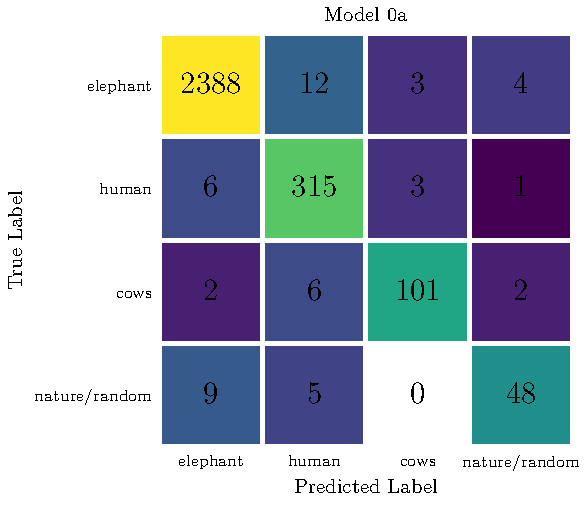
\includegraphics[width=1\linewidth]{good_cm.pdf} 
    \end{subfigure}
    \begin{subfigure}{0.5\textwidth}
        \centering
        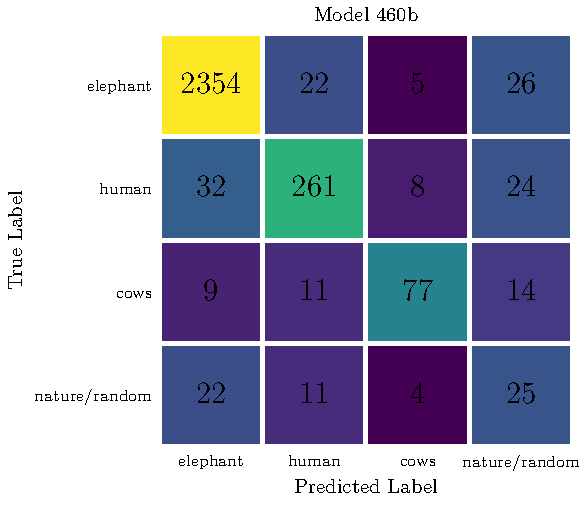
\includegraphics[width=1\linewidth]{bad_cm.pdf}
    \end{subfigure}
    \caption{Confusion matrices of \textit{0a} model (left) and \textit{460b} model (right)}
    \label{double_cm}
\end{figure}


\subsection{ Comparison with Edge Impulse model}

Choose one, or few model configurations and make a model in EI.

Describe how did you build Edge Impulse model, maybe mention transfer learning (might be extra work, you did not write about theory)




\section{ On device performance testing}
Describe setup

To profile execution of our code we first wrote a timer driver based on a Arm's systick timer, however we later decided to use data watch trigger (DWT).
DWT does not use interrupts, therefore it does not introduce overhead of calling interrupt routines like systick timer does.


      how are you timing, 

\subsection{ Comparison of different optimization options}
\subsection{ Comparison of performance of selected models}
    Transfer learning could be interesting here, bigger number of parameters and takes less time.






\section{ Power profiling of an embedded early warning system}
- [ ] Power consumption test of whole setup, 
      PIR wakes up wisent, 
      wisent turns on stm32f7 and flir, 
      which makes a picture, does inference, reports result and wisent sends the result. 
      Otii image of consumption with marked sections.(shouldnt be hard)

\subsection{ Battery life estimations}
Based on numbers and different scenarios estimate how long would this last with different batteries.
